\documentclass[10pt, letterpaper]{article} 
% \usepackage{fullpage}
\usepackage[top=1in, bottom=1in, left=0.5in, right=0.5in, paperwidth=8.5in, paperheight=11in]{geometry} % this gives you a lot of control, you can also use margin= for all sides
% this changes the margins of the paper
\usepackage{amsfonts} % give additional math notation
\usepackage{amssymb}
\usepackage{amsmath}
\usepackage{graphicx} % this is if you want to insert an image
\usepackage{float} % for capital H
\def\eq1{v=\frac{x}{3x^2+x+1}}
% this is called a macro (sort of like a global variable) called eq1 and the value is inside the curly brackets

\newcommand{\set}[1]{\setlength\itemsep{#1em}}


\begin{document}
 
\textbf{Critical Thinking Questions}
\begin{figure}[H] % used a lot for images
	\centering
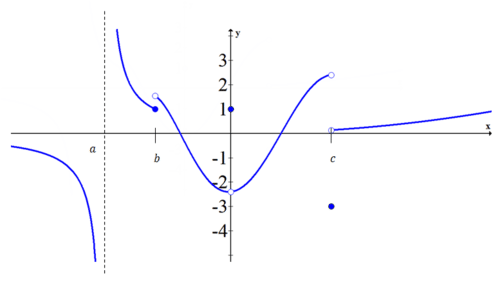
\includegraphics[width=0.5\textwidth]{limit} % dont have to put .png or .jpeg. this is how you include an image
% 0.5\textwidth just means 50 percent of the text width
\caption{The Squeeze Theorem} % this how to add the caption
\end{figure}

\begin{enumerate}
\set{1}
\item Let's examine the function $\eq1$ % it worked as you can see here
\item This is the symbol for all real numbers: $\mathbb{R}$
\item This is the symbol for the set of integers: $\mathbb{Z}$
\item This is the symbol for the set of rational numbers: $\mathbb{Q}$
\item Is it possible for a sequence to converge to two different numbers? If so, give an example. If not, explain why not.
\item Explain how to use partial sums to determine if a series converges or diverges. Give an example
\item Explain why $\int\limits_{1}^{\infty} f(x)\,dx$ and $\sum\limits_{n=1}^{\infty} a_n$ need not converge to the same value, even if they are both convergent.
\item  In your own words, explain the Alternating Series Remainder Theorem. How is this theorem useful?
\item Explain the difference between absolute and conditional convergence. Give an example of each.
\item The Ratio Test is inconclusive if $\displaystyle{\lim\limits_{n \to \infty} \left| \frac{a_{n+1}}{a_n} \right| =1}$. Give an example of one convergent series and one divergent series for which $\displaystyle{\lim\limits_{n \to \infty} \left| \frac{a_{n+1}}{a_n} \right| =1}$. Explain how you determined your examples.
\end{enumerate}

\end{document}



